\spacing{1.25}

Se estudiar\'a la componente mu\'onica de la distribuci\'on lateral en cascadas atmosf\'ericas producidas por rayos c\'osmicos de altas energ\'ias. Para ello, con el sistema AIRES, se realizar\'an dos grupos de simulaciones por cada modelo de interacciones hadr\'onicas: el primer grupo de cascadas producidas por protones y el segundo de cascadas producidas por n\'ucleos de hierro. Cada grupo consistir\'a en aproximadamente 2000 cascadas con energ\'ias primarias del orden de los TeV.

\section{Características de las cascadas}
Se simular\'an cascadas producidas por rayos cósmicos de energías entre $10^{12}$ y $10^{14}$ eV, en la ubicaci\'on del observatorio HAWC en Puebla, M\'exico, con latitud de 19$^{o}$ y altura de 4100 m sobre el nivel del mar. Se considerar\'an direcciones de incidencia con ángulo zenital \ccnote{creo que por el entorno de HAWC esto podr\'ia cambiar} entre 0$^{o}$ y 70$^{o}$ y ángulo azimutal distribuido isotrópicamente entre 0$^{o}$ y 360$^{o}$. Se utilizar\'an tres modelos de interacciones hadrónicas de altas energías; Sibyll 2.3d, EPOS-LHC y QGSJETII-04. Los tres modelos son ampliamente utilizados para simulaciones de cascadas atmosf\'ericas y han presentado discrepancias con las observaciones de la componente mu\'onica. Se realizar\'an simulaciones de cascadas producidas por protones y por n\'ucleos de hierro. \\
	 
\section{Software para simulaciones de altas energías}
El sistema AIRES (AIR shower Extended Simulations) es un conjunto de programas para simular cascadas atmosféricos extendidos desarrollado por el Departamento de Física de la Universidad Nacional de La Plata y el Instituto de Física La Plata. AIRES está diseñado de manera modular para facilitar el intercambio entre los modelos de distintos aspectos de las simulaciones. El código completo de AIRES incluye los paquetes de interacciones hadrónicas EPOS 1.99, EPOS LHC, QGSJET-II-03, QGSJET-II-04, SIBYLL 2.1, SIBYLL 2.3, y SIBYLL 2.3c, así como las rutinas para evaluar el campo geomagnético. En síntesis, el sistema AIRES consiste en:
	\begin{itemize}
	\item Los programas de simulación principales (AiresEPLHC, AiresEP199, AiresQIIr03, AiresQIIr04, AiresS21, AiresS23, AiresS23c), cada uno conteniendo la interfaz para un paquete de interacciones hadrónicas.
	\item El programa resumen (AiresSry), diseñado para procesar parte de los datos generados por los programas de simulación.
	\item El programa de conversión de formato IDF (\textit{internal dump file}) a ADF (\textit{portable dump file}) (AiresIDF2ADF).
	\item Una librería de auxiliares para procesar los archivos de salida de los programas de simulación (libAires.a)
	\item El \textit{AIRES runner system}, para facilitar el trabajo con AIRES en ambientes UNIX. 
	\end{itemize}
	
	\subsection{Sistema de coordenadas}
	\begin{wrapfigure}{r}{0.3\textwidth}
	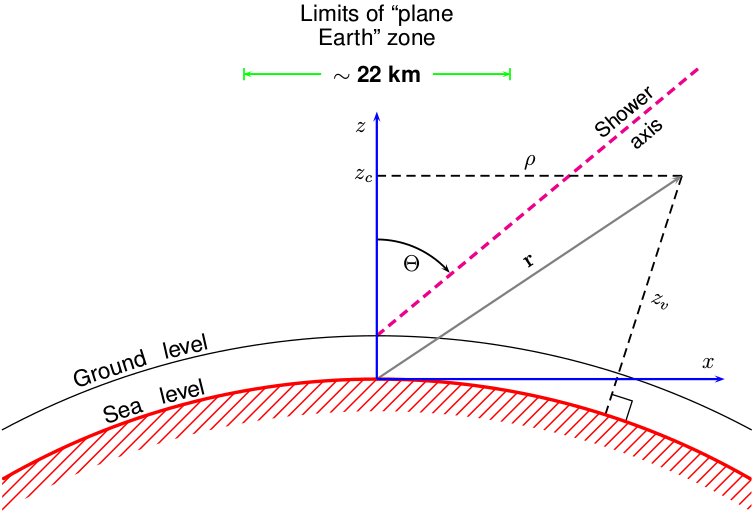
\includegraphics[width=0.3\textwidth]{Figuras/coordinates} 
	\caption{Esquema del sistema de coordenadas utilizado en AIRES.}
	\label{fig:coordinates}
	\end{wrapfigure}		
	El sistema de coordenadas de AIRES es un sistema cartesiano con el origen al nivel del mar en la ubicación proporcionada por el usuario, el plano $xy$ se posiciona horizontalmente; el eje $x$ apunta hacia el norte magnético, el eje $y$ hacia el Este y el eje $z$ hacia arriba. En la figura \ref{fig:coordinates} se muestra una representación esquemática del sistema coordenado, incluyendo el nivel del suelo y el nivel de inyección, éstos se refieren a superficies esféricas concéntricas con la superficie del nivel del mar. El eje del cascada se define como una línea recta que pasa por la intersección del nivel del suelo con el eje $z$, con un ángulo cenital $\Theta$ y un ángulo azimutal $\Phi$.
	
	\subsection{Atmósfera}
	AIRES utiliza el modelo basado en datos experimentales \textit{US standard atmosphere} como modelo predeterminado. En este modelo, la composición de la atmosféra es $78.47\%$ N, $21.05\%$ O, $0.47\%$ Ar y $0.03\%$ otros elemento. El perfil de densidad isotérmico de la forma
	\begin{align*}
	\rho (h) = \rho_0 e^{-gMh/RT},
	\end{align*}
	
	se adapta a los valores de la \textit{US standard atmosphere}. En AIRES el modelo se extiende hasta una altura $h_{max} \sim 420$ km, después de la cual se considera que la densidad es cero. Se utiliza una parametrización de la profundidad atmosférica vertical $X_v$; dividiendo la atmósfera en $L$ capas, $X_v (h)$ se define por 
	\begin{align}
	X_v (h) = \begin{cases}
	a_l + b_l e^{-h/c_l} & h_l \leq h < h_{l+1} \\
	a_L - b_L (h/c_L) & h_L \leq h < h_{L+1} \\
	0 & h \geq h_{L+1}.
	\end{cases}
	\end{align}
	
	La profundidad atmosférica inclinada (\textit{slant}) $X_s$ depende del ángulo cenital y cuando no se toma en cuenta la curvatura de la Tierra, se relaciona con $X_v$ de la siguiente manera:
	\begin{align}
	X_s (h) = \frac{X_v (h)}{\cos(\Theta)}.
	\end{align}
	
	\subsection{Campo geomagnético}
	El campo magnético de la Tierra $\vb{B}$ se define por su intensidad $F$; su inclinación $I$, que se define como el ángulo entre el plano horizontal y el vector $\vb{B}$; y su declinación $D$, que se define como el ángulo entre la componente horizontal ($H$) de $\vb{B}$ y el norte geográfico. Las componentes cartesianas de $\vb{B}$ con respecto al sistema coordenado de AIRES son 
	\begin{align}
	B_x &= F \cos I, \\
	B_y &= 0, \\
	B_z &= -F \sin I.
	\end{align}	 
	
	Hay dos maneras de especificar el campo geomagnético en AIRES; la primera es ingresando manualmente los valores de $F$, $I$ y $D$, y la segunda es ingresando las coordenadas geográficas del lugar y la fecha para evaluar el campo magnético utilizando el modelo \textit{International Geomagnetic Reference Field} (IGRF).  	
	
	\subsection{Modelos de interacción}
	En AIRES se toman toman en cuenta los procesos más relevantes; procesos electrodinámicos como producción de pares (para $e^{\pm}$ y $\mu^{\pm}$), \textit{Bremsstrahlung}, efecto fotoeléctrico y efecto Compton; procesos hadrónicos como colisiones hadrón-núcleo, reacciones fotonucleares y fragmentación nuclear; procesos de decaimiento y procesos de propagación. Cada interacción posible está caracterizada por su sección eficaz $\sigma_i$ o por su camino libre medio $\lambda_i$. Los caminos libres medios dependen del tipo de interacción y los parámetros instantáneos de la partícula. AIRES puede calcular $\lambda_i$ analíticamente para interacciones a bajas energ\'ias con el algoritmo de divisi\'on de Hillas o con un modelo de fragmentaci\'on nuclear dependiendo del tipo de interacci\'on. A altas energ\'ia debe recurrir a los modelos externos basados en datos experimentales. 
	
	\subsection{Estructura de los programas de simulación}
	Un cascada se origina cuando un rayo cósmico interactúa con la atmósfera terrestre, donde se producen partículas secundarias que se propagan y pueden interactuar de manera similar produciendo más partículas. Eventualmente la multiplicidad de partículas llega a un máximo, después del cuál  la cascada empieza a atenuarse. En AIRES todo este proceso se simula de la siguiente manera \cite{Sciutto2002}:
	\begin{itemize}
	\item Se definen arreglos vacíos destinados a almacenar los datos de las características de las partículas.
	\item Las partículas pueden moverse por la atmósfera en un volumen delimitado por la superficie de inyección, el suelo y planos verticales que delimitan la región de interés.
	\item La primera acción es añadir a un arreglo la entrada correspondiente a la partícula inicial, ésta se localiza inicialmente en la superficie de inyección y su dirección de movimiento define el eje de la cascada.
	\item Las entradas respectivas a cada partícula se actualizan primero evaluando las probabilidades de todas las interacciones posibles.
	\item Se selecciona entre las posibles interacciones utilizando un método estocástico.
	\item Se procesa la interacción; la partícula se mueve una cierta distancia dependiente de la interacción seleccionada y luego se generan los productos de dicha interacción. Se agregan a los arreglos las entradas de las nuevas partículas creadas.
	\item En el caso de las partículas cargadas, se modifica la energía para tomar en cuenta pérdidas por ionización.
	\item Las entradas de partículas pueden removerse (1) si su energía es menor que cierto límite, (2) si alcanza el nivel del suelo, (3) si alcanza la superficie de inyección hacia arriba y (4) si horizontalmente sale de la región de interés.
	\item Se verifica que todas las entradas de partículas de los arreglos se hayan procesado; cuando se hayan procesado se completa la simulación d la cascada.
	\end{itemize}	
	
	\subsection{Muestreo de partículas}
	Para chubascos iniciados por partículas de ultraalta energía, el número de partículas secundarias producidas es tan grande que la tarea computacional de propagarlas todas es imposible; para poder realizar las simulaciones se emplea un mecanismo de muestreo que permite propagar únicamente un fracción representativa del total de partículas secundarias. AIRES utiliza una extensión del \textit{Hillas thinning algorithm} \cite{Kobal2001}. \\
	
	Considerando un proceso donde una partícula primaria $A$ genera un conjunto de $n$ secundarios, éstos son propagados con cierta probabilidad $P_i$. El algoritmo de Hillas consiste en establecer una constante $E_{th}$ llamada \textit{thinning energy}; para incorporar a los secundarios $B_i$ en la propagación se compara la energía de la partícula primaria $E_A$ con $E_{th}$: si $E_A \geq E_{th}$, entonces los secundarios de aceptan con una probabilidad
	\begin{align}
	P_i = \begin{cases}
	1 & \text{ si } E_{B_i} \geq E_{th} \\
	\frac{E_{B_i}}{E_{th}} & \text{ si } E_{B_i} < E_{th}.
	\end{cases}
	\end{align}
	Por el contrario, si $E_A < E_{th}$ sólo una partícula secundaria se conserva, lo que asegura que una vez se alcance $E_{th}$ el número de partículas no se incrementa. El algoritmo utilizado por AIRES es una extensión de lo descrito anteriormente, pero éste incluye características adicionales para disminuir las fluctuaciones estadísticas.

\singlespacing